\newpage
\section{Introduction}
MetaDoc is created as a way to securely transport data between a server and 
sites. It is created to improve the flow of information between \gls{hpc} sites
and Uninett Sigma \cite{improvingflow}.

MetaDoc consists of a client, running at the site, and a server running at the
Metacenter. MetaDoc takes care of authenticating the client on the server,
packing and unpacking the data to and from \gls{xml}, and transporting the data
securely between client and server. 

If you wish to get the client up and running as quickly as possible, the
MetaDoc Client Quick Start Guide is a good place to start
\cite{quick_start_guide}.

\begin{figure}[h!]
    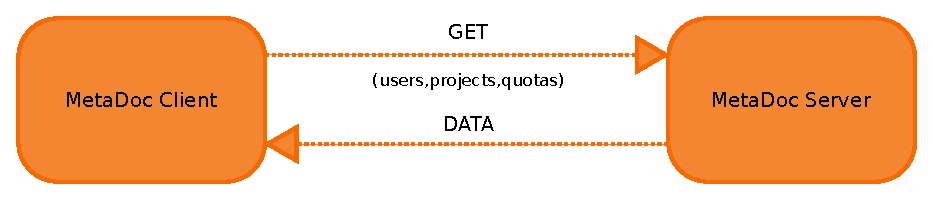
\includegraphics[width=\textwidth]{img/get_data}
    \caption{Client requesting data from server}
    \label{fig:get_data}
\end{figure}

Figure \ref{fig:get_data} shows how the client requests data from the server.
The MetaDoc client provides the interface for retrieving this data, and it is
then up to the site to decide how to handle the recieved data. 

\begin{figure}[h!]
    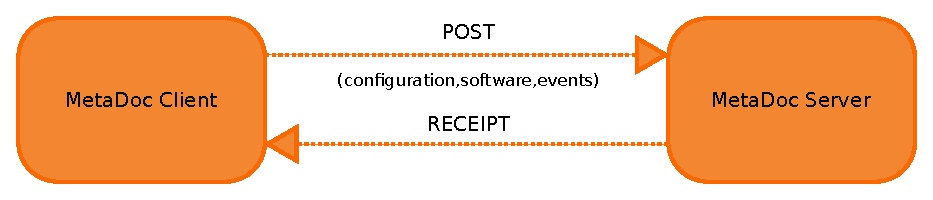
\includegraphics[width=\textwidth]{img/post_data}
    \caption{Client sending data to server. Server returns a receipt for
    recieved data.}
    \label{fig:post_data}
\end{figure}

In figure \ref{fig:post_data}, data is sent from the client to the server. On
recieving the data, the server will return a receipt, telling the client that
the data has been processed and accepted or rejected. 

In section \ref{sec:overview}, an overview of the MetaDoc client is given. It
explains what is done by the standard client, and how the client can run. 

Section \ref{sec:client_api} explains how to customize the MetaDoc client in
order to process the data sent between the client and server. 

Section \ref{sec:server_api} goes through the server side API. It explains how
the server acts in response to requests by the MetaDoc client. 

The \gls{xml} document used to send data between the client and server is
explained in section \ref{sec:xmldoc}. 

Section \ref{sec:useful_classes} describes some useful classes and modules
provided by the MetaDoc client for use when extending the client to send or
recieve more data. 

A guide to extending the client is given in section \ref{sec:extending}. This
is a step for step guide that explains what is needed in order for the client
to send or recieve more data. 

The information flow between client and server is explained in more detail in
section \ref{sec:information_flow}.

An explanation of possible errors that may occour during usage of the MetaDoc
client is given in section \ref{sec:errors}. 
